\documentclass[12pt, a4paper, one side]{article}
\usepackage[utf8]{inputenc}
\usepackage[french]{babel}
\usepackage{biblatex}
\usepackage{listings}
\usepackage{xcolor}
\usepackage{hyperref}
\usepackage{graphicx}
\usepackage{minted}

\bibliography{reference}

\usepackage{comment}

\lstset{
    basicstyle=\itshape,
    xleftmargin=3em,
    literate={->}{$\rightarrow$}{2}
        {^}{$\uparrow$}{1}
        {↓}{$\downarrow$}{1},
    morekeywords={method_body},
    basicstyle=\small
}

\definecolor{codegreen}{rgb}{0,0.6,0}
\definecolor{codegray}{rgb}{0.5,0.5,0.5}
\definecolor{codepurple}{rgb}{0.58,0,0.82}
\definecolor{backcolour}{rgb}{0.95,0.95,0.92}

\lstdefinestyle{mystyle}{
    commentstyle=\color{codegreen},
    keywordstyle=\color{magenta},
    numberstyle=\tiny\color{codegray},
    breakatwhitespace=false,
    breaklines=true,
    captionpos=b,
    keepspaces=true,
    numbers=left,
    numbersep=5pt,
    showspaces=false,
    showstringspaces=false,
    showtabs=false,
    tabsize=2,
    extendedchars=true
}

\newcommand{\paragraphln}[1]{\paragraph{#1}\mbox{}\\}



\title{Documentation de l'extension}
\author{}
\date{}

\begin{document}

    \maketitle

    \begin{center}
        Valentin Laclautre, Anthony Dard, Damien Trouche, Martin Gangand, Basel Darwish Jzaerly
    \end{center}

    \tableofcontents

    \newpage

    \section{Spécifications}

    A noter que vous devez disposez au minimum de la version 1.8 de java pour
    pouvoir faire tourner les programmes deca compilés en bytecode java.

    \subsection{Compilation de programmes Deca en executable pour la JVM}
    \subsubsection{Commande decac}
    \textbf{decac [[-p $\mid$ -v $\mid$ -java] [-n] [-r X] [-d]* [-P] [-w] $<$fichier deca$>$...] $\mid$ [-b]}
    \\

    L'option -java spécifie au compilateur qu'on souhaite compiler un programme Deca en executable pour la machine virtuelle Java.
    Ainsi, on obtient avec cette obtion un fichier .class executable par la JVM au lieu d'un fichier .ass (executable IMA). Les conventions de nommage sont les mêmes, c'est-à-dire que le nom du fichier compilé est celui du programme Deca, seule l'extension du fichier change.

    Cependant il y a quelques restrictions. En effet, l'utilisation de code Java dans une méhode Deca impose une compilation vers la JVM (une erreur est renvoyée sinon). De plus la compilation vers la JVM impose qu'il n'y ai pas de méthode en Assembleur. (cf Limitations pour plus de précisions)

    \subsubsection{Spécification de compilation}
    La compilation se fait de la même manière que pour la machine IMA au detail près qu'au lieu d'appeler nos méthodes de compilation pour la machine abstraite IMA, le compilateur utilise la bibliothèque ASM\cite{ASM} pour la génération du bytecode.

    \subsubsection{Compiler un programme Deca}

    Pour compiler un fichier deca, il suffit simplement de taper : \newline
    \textbf{decac -java path/fich.deca}

    \subsubsection{Fichiers créés par la compilation}

    Lors de la compilation d'un fichier deca, un premier fichier correspondant
    au programme principale portant le même nom que le fichier deca est créé (mais
    avec l'extension .class au lieu de .deca), puis un fichier portant le nom
    MethodBody est créé. Ce fichier permer de gérer l'insertion de java en deca
    (pour plus de précision, veuillez regardez la section consacrée). Enfin pour
    chaque classes deca contenue dans ce fichier, un fichier .class est créé avec
    le même nom que le nom de la classe. Ce fichier correspond au bytecode de la
    classe deca.

    \subsubsection{Exécuter des fichiers deca}

    Après avoir compilé un fichier deca (nommé pour l'exemple \textit{fich.deca})
    on aimerai pouvoir l'exécuter. Pour cela, il faut se placer dans le répertoire
    du fichier deca (là où les fichiers .class se sont créés) et il faut taper :
    \newline \textbf{java fich}. On peut aussi taper \textbf{java -cp path fich} où path correspond au chemin du fichier deca.

    \subsection{Appel de code Deca en Java}

    Après avoir créée une classe en deca, et l'avoir compilé en un fichier .class,
    il est possible de l'instancier dans une classe java. Malgré tout, pour pouvoir
    faire cela, il faut placer le fichier java et le fichier deca au même endroit.
    Après l'avoir instancié, on peut l'utilisé de la même maniere qu'une classe
    java, et faire appel à des méthodes ou des champs de la classe deca.

    \subsubsection{Exemple de Deca vers Java}

    Dans cet exemple, il y a 2 fichiers: un fichier deca comportant une classe, et
    un fichier java instanciant cette classe. \newline
    \newpage
    \textbf{Math.deca}
    \begin{minted}{java}
        class Math {
        	int add(int a, int b) {
        		return a + b;
        	}

        	int mult(int a, int b) {
        		return a * b;
        	}
        }
    \end{minted}

    \textbf{Main.java}
    \begin{minted}{java}
        class Main {
        	public static void main(String[] args) {
        		Math m = new Math();
        		int c = m.add(1, 2);
        		System.out.println(c);
        		c = m.mult(5, 3);
        		System.out.println(c);
        	}
        }
    \end{minted}

    Pour compiler, il ne reste plus qu'à copier les lignes suivantes :
    \begin{minted}{bash}
        $ decac -java Math.deca
        $ javac Main.java
    \end{minted}

    Ces deux commandes compilent dans un premier temps le programme deca, puis
    dans un second temps le programme principale java. Enfin, il ne reste plus qu'à
    exécuter le programme :

    \begin{minted}{bash}
        $ java Main
        3
        15
    \end{minted}

    \subsubsection{Intérêt d'avoir du code Deca vers Java}

    Cela permet un portage très simple pour les développeurs ayant décidé
    d'utiliser le langage java et ayant besoin d'utiliser une éventuelle librairie deca.
    Le langage deca étant neuf, un portage du langage vers java serait un atout attrayant pour les développeurs.

    \subsection{Appel de code Java en Deca}
    Cette section précise les spécifications liées à l'appel de code Java en Deca.
    \subsubsection{Grammaire Deca pour l'appel de code Java}
    Une règle est ajoutée à la passe 3 pour prendre en compte les méthodes "Java"
    \begin{lstlisting}
method_body↓env_type↓env_exp↓env_exp_params↓class↓return
            -> MethodJavaBody [ StringLiteral ]
    \end{lstlisting}

    \subsubsection{Utilisation}
    L'utilisation de l'appel de code Java en Deca est très similaire à l'appel de code assembleur. En effet, il suffit de déclarer une méthode de la même manière, c'est-à-dire une méthode dont le corps est une chaîne de caractères contenant du code Java et en utilisant le mot clé 'java' à la place de 'asm'.
    \\

    Il est possible d'envoyer une valeur qui se trouve dans le code deca vers le code java en utilisant les paramètres de la méthode deca. Un exemple d'utilisation se trouve dans src/test/deca/codegen/valid/custom/extension/*.
    \\

    Enfin, il est utile de rappeler qu'il est possible de compiler une classe écrite en deca et puis utiliser le bytecode généré dans un programme java. On note que le fichier deca source doit être dans le même répertoire que le fichier java afin que la compilation fonctionne. C'est une limitation de deca.

    \section{Analyse bibliographique}
    Dans cette section nous allons donner des détails techniques sur la  \textbf{Java virtual machine JVM}.

    \begin{figure}[h]
        \centering
        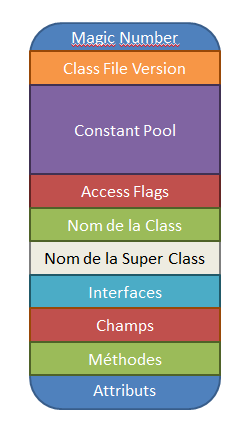
\includegraphics[scale=0.80]{JavaInternal.png}
        \caption{L'architecture de fichier .class \cite{ref_DexFormatvsJavabytecode}}
        \label{fig1}
    \end{figure}


    Les fichiers .class sont les fichiers exécutables par la machine virtuelle java. Chaque fichier .class contient les informations concernant une et une seule classe en Java. Dans ce fichier on trouve les instructions écrites en bytecode qui seront exécutées par la JVM. Nous présentons par la suite quelques détails, mais pour plus de détails il faut regarder les spécifications du java \cite{ref_specifications_java} .

    \subsection{Magic number}
    Il s'agit d'un attribut identifiant les fichiers d'execution Java \cite{ref_DexFormatvsJavabytecode}.

    \subsection{Class file version}
    Permet de déterminer la version minimum de la machine virtuelle de java qui pourra exécuter ce fichier. Donc si la version du fichier est supérieure à celle de la JVM, la machine virtuelle ne pourra pas l'exécuter.

    \subsection{Constant Pool}
    C'est une table qui contient toutes les constantes de la classe. Ces constantes peuvent être de types différents tels que \textbf{String},\textbf{Integer}, \textbf{Float}... etc. Par exemple, lorsque le fichier .java contient une variable qui a pour valeur 123456, cette table contiendra une case référencée par un indice et cette case stocke la valeur. De façon similaire, une chaîne de caractères telle que "ma belle chaîne de caractère" sera stockée dans une autre case dans la table.

    \subsection{Access Flags}
    Contient les informations sur l'accessibilité de la classe.

    \subsection{Class Name}
    On y trouve le nom de la classe.
    \subsection{Super Class Name}
    On y trouve le nom de la classe mère.

    \subsection{Interface}
    Si la classe implémente une interface, alors le nom de l'interface sera mentionné ici.

    \subsection{Champs}
    Les champs de la classe sont présentés ici avec leur niveau d'accessibilité private,protected ou public avec son nom et son type.

    \subsection{Methods}
    De façon similaire aux champs, chaque méthode est décrite par son niveau d'accessibilité, son nom, les types de ses paramètres et le type de retour.


    \section{Conception}
    \subsection{Documentation de conception}
    \subsubsection{Structure globale}
    \subsubsection{Choix d'implémentation}
    \subsection{Algorithmes utilisés}

    \section{Validation}
    \subsection{Protocole de validation}
    \subsection{Résultats}

    \section{Limitations}
    \subsection{Compatibilité Java-Deca}

    \newpage
    \printbibliography

\end{document}
